\documentclass[addpoints,12pt]{exam}
\newcommand{\ds}{\displaystyle}
\usepackage[margin=0.8in]{geometry}
\usepackage{subcaption}
\usepackage{tikz}

\usepackage{amssymb,amsmath,graphicx,wrapfig,verbatim,wasysym, enumitem,psfragx,color}
\usepackage{multicol}

\usepackage{xpatch}

\makeatletter
\xpatchcmd{\@fillin@relay}
  {\hbox to #1{\hrulefill}\fi}
  {\hbox{\framebox[#1]{\rule{0pt}{2ex}}}\fi}
  {}{}
\makeatother

%\usepackage{fancyhdr}
%\setlength{\headheight}{13.6pt}
%\pagestyle{fancy}
%\lhead{Math 222}
%\chead{ Midterm 1 }
%\rhead{Spring 2022}

\def\FillInBlank{\rule{3truein} {.01truein}}




% Choose one option (bubbles)
\newcommand{\chooseone}{{\Large$\Circle$\ \ }}
% Choose multiple options (squares)
\newcommand{\choosemany}{{\Large$\Square$\ \ }}


\newcommand{\myleft}{\makebox[.4\textwidth]{First Name:\enspace\hrulefill}}
\newcommand{\myright}{\makebox[.4\textwidth]{Last Name:\enspace\hrulefill}}
\header{\oddeven{\myleft}{}}
    {}
    {\oddeven{\myright}{}}

\footrule

\footer{Math 211}
     {Midterm 1 Practice Exam}
     {Page \thepage\ of \numpages}

\begin{document}

\begin{questions}


\question Clearly mark the correct answer(s) for each of the following by completely filling in the
appropriate bubble. \textbf{No justification is needed.}


\begin{parts}

\part[2] \textbf{(Multiple Choice-Choose one)} Where does $f(x)=x-3\sqrt{x}$ have a horizontal
tangent line?

\begin{itemize}[label={}]
\item \chooseone $x=0$
\item \chooseone $x=1$
\item \chooseone $x=\frac{1}{2}$
\item \chooseone $x=\frac{9}{4}$
\item \chooseone None of the above.
\end{itemize}

\medskip




\part[2] \textbf{(True/False)} If $f(x)=x^2+2$ and $g(x)=4x+3$, $f(g(x))=g(f(x))$.

\begin{itemize}[label={}]
\item \chooseone True
\item \chooseone False
\end{itemize}

\vfill




\part[2] \textbf{(Choose all that apply)} Given the graph of $y=f(x)$ below, where is $f(x)$
discontinuous?
\begin{itemize}[label={}]
\item \choosemany $x=-1$
\item \choosemany $x=1$
\item \choosemany $x=3$

\item \choosemany None of the above.
\end{itemize}

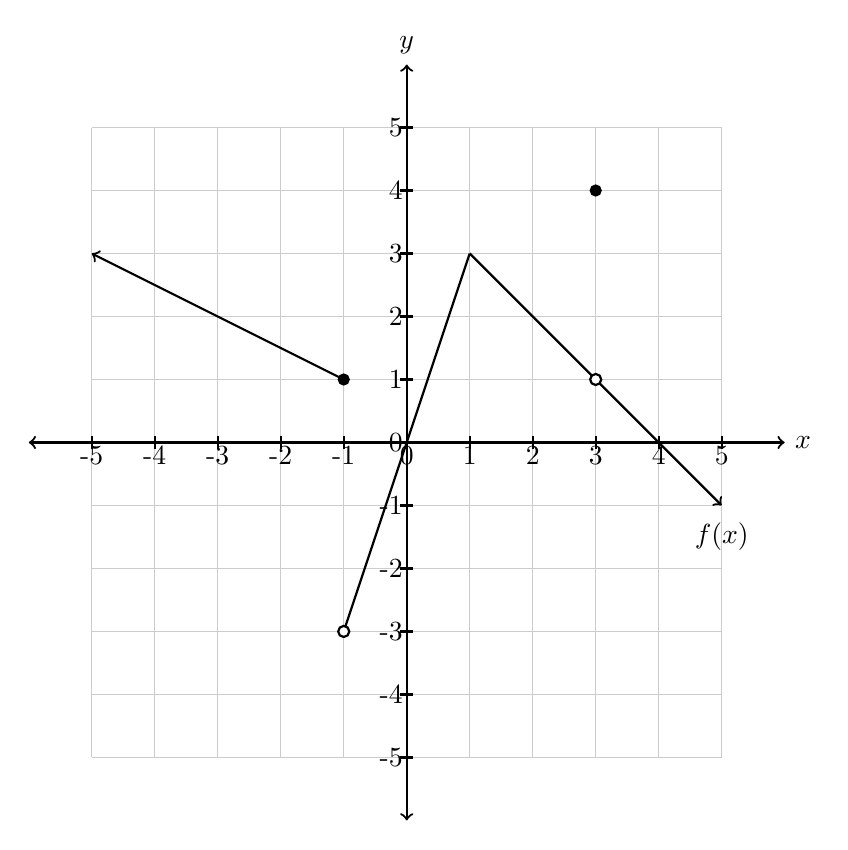
\begin{tikzpicture}[scale=.8]
\draw[gray!40] (-5, -5) grid[step=1] (5, 5);
\draw[<->,thick,black] (-6,0)--(6,0) node[right]{$x$};
\draw[<->, thick,black] (0,-6)--(0,6) node[above]{$y$};
\foreach \x in {-5,-4,...,5}
\draw[thick] (\x,-.1) --(\x,.1) node[below]{\x};
\foreach \y in {-5,-4,...,5}
\draw[thick] (-.1,\y) --(.1,\y) node[left] {\y};
\draw[domain=1:5,samples=100, thick,->] plot ({\x},{-(\x+1)+5});
\draw[domain=-1:1,samples=100, thick,-] plot ({\x},{3*\x});
\draw[domain=-5:-1,samples=100,thick,<-] plot ({\x},{(-\x/2+0.5});
\draw[fill=black] (3,4) circle[radius=0.25em];
\draw[fill=black] (-1,1) circle[radius=0.25em];
\draw[fill=white,thick] (3,1) circle[radius=0.25em];
\draw[fill=white,thick] (-1,-3) circle[radius=0.25em];
\node at (5,-1.5) {$f(x)$};
\end{tikzpicture}




\vfill

\end{parts}

\newpage


\newpage


\question Calculate the derivative of each function. You do not need to simplify your answer.

\begin{parts}




\part[5] $\ds g(x)=x^3-3(x^2+10^2)$
\vspace{2in}

\part[5] $\ds r(x)=\sqrt{x+\sqrt{x}}$

\vspace{2in}

\part[5] $\ds f(t)=\frac{7}{t^{4/3}}-8t$

\vspace{2in}

\part[5] $f(x)=(x^3+2x-7)(x^4-3x^2+x)$

\vspace{2in}




\end{parts}

\newpage


\question Given the graph of $f(x)$ and the graph of $g(x)$ below:


\begin{minipage}{.45\textwidth}
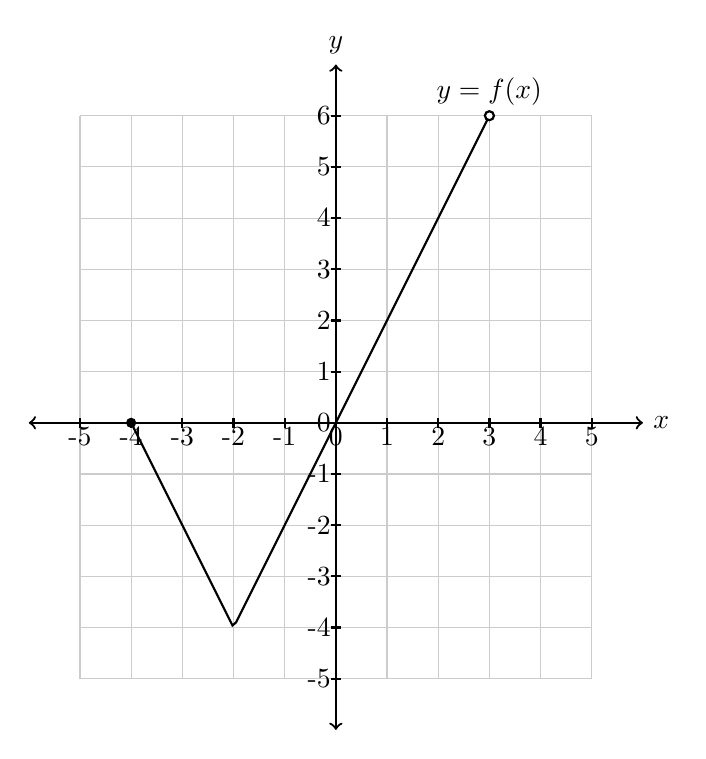
\begin{tikzpicture}[scale=.65]
\draw[gray!40] (-5, -5) grid[step=1] (5, 6);
\draw[<->,thick,black] (-6,0)--(6,0) node[right]{$x$};
\draw[<->, thick,black] (0,-6)--(0,7) node[above]{$y$};
\foreach \x in {-5,-4,...,5}
\draw[thick] (\x,-.1) --(\x,.1) node[below]{\x};
\foreach \y in {-5,-4,...,6}
\draw[thick] (-.1,\y) --(.1,\y) node[left] {\y};
\draw[domain=-4:3,samples=100, thick,-] plot ({\x},{2*abs(\x+2)-4})node[above]{$y=f(x)$};
\draw[fill=black] (-4,0) circle[radius=0.25em];
\draw[fill=white,thick] (3,6) circle[radius=0.25em];
\end{tikzpicture}
\end{minipage}
\begin{minipage}{.45\textwidth}
\begin{tikzpicture}[scale=.65]
\draw[gray!40] (-5, -5) grid[step=1] (5, 5);
\draw[<->,thick,black] (-6,0)--(6,0) node[right]{$x$};
\draw[<->, thick,black] (0,-6)--(0,6) node[above]{$y$};
\foreach \x in {-5,-4,...,5}

\draw[thick] (\x,-.1) --(\x,.1) node[below]{\x};
\foreach \y in {-5,-4,...,5}
\draw[thick] (-.1,\y) --(.1,\y) node[left] {\y};
\draw[domain=-3:-1,samples=100, thick,-] plot ({\x},{3*\x+5});
\draw[domain=-1:5,samples=100, thick,-] plot ({\x},{-1/3*\x+5/3})node[above]{$y=g(x)$};
\draw[fill=white,thick] (-1,2) circle[radius=0.25em];
\draw[fill=black] (-3,-4) circle[radius=0.25em];
\draw[fill=black] (5,0) circle[radius=0.25em];

\end{tikzpicture}

\end{minipage}

\begin{parts}
\part[2] Give the domain and range of $f(x)$. Use interval notation.
\vspace{1in}

\part[2] Give the domain and range of $g(x)$. Use interval notation.
\vspace{1in}

\part[2] What is $g(f(-3))$?
\vspace{1in}

\part[2] Find $F'(2)$, where $F(x)=f(x)g(x)$. You do not need to simplify your final numerical
answer.
\vspace{1in}
\end{parts}

\newpage




Find each limit. Show all work. Simplify your final answers.

\begin{parts}

\part[4] $\displaystyle\lim_{x\to 1} \dfrac{x^2-4x+4}{x^3+5x^2-14x}$

\vfill


\part[4] $\displaystyle\lim_{x\to 4} \dfrac{x^2+x-20}{2x^2-6x-8}$

\vfill

\end{parts}

\newpage

\question[11] Find an equation for the tangent line of the function $f(x)=x-2x^2$ at $x=3$. Show
all work.

\newpage

\question[8] Find $g''(x)$ of $g(x)=4\sqrt{x}-\dfrac{1}{x^2}$. You do not need to simplify your final
answer. Show all work.


\newpage




\question Suppose a USB manufacturer finds that the cost of producing $x$ total USBs is
$C(x)=40+24x^{1/3}$.
\begin{parts}
  \part[4] Find the marginal cost function $MC(x)$ and evaluate it at $x=8$. Simplify your
answer.
  \vfill

  \part[5] Find the marginal average cost function $MAC(x)$ and evaluate it at $x=8.$ Simplify
your answer.
   \vfill
\end{parts}


\newpage


\question Given the graph of $f(x)$ below, find each limit. Write $\infty, -\infty$, or DNE if
applicable.

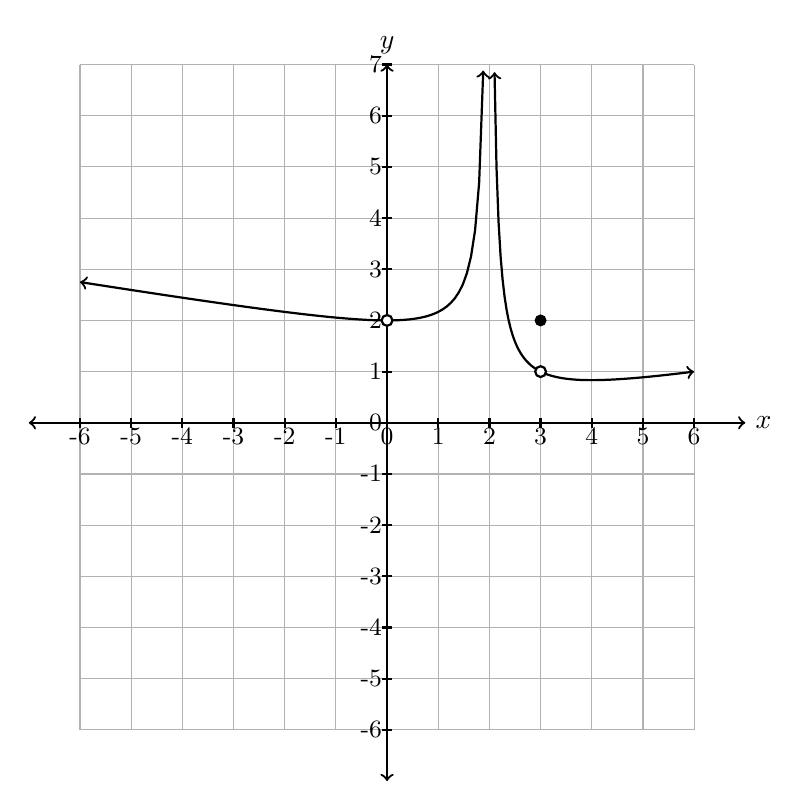
\begin{tikzpicture}[scale=.65]
\draw[gray!60] (-6, -6) grid[step=1] (6, 7);
\draw[<->,thick,black] (-7,0)--(7,0) node[right]{$x$};
\draw[<->, thick,black] (0,-7)--(0,7) node[above]{$y$};
\foreach \x in {-6,-5,...,6}
\draw[thick] (\x,-.1) --(\x,.1) node[below] {\small \x};

\foreach \y in {-6,-5,...,7}
\draw[thick] (-.1,\y) --(.1,\y) node[left] {\small \y};
 \draw[domain=-6:1.88,samples=100, thick,<->] plot ({\x},{-\x*\x/(\x-2)/6+2});
 \draw[domain=2.1:6,samples=100,thick,<->] plot ({\x},{\x*\x/(\x-2)/6-1/2});
\draw[fill=white,thick] (3,1) circle[radius=0.3em];
\draw[fill=white,thick] (0,2) circle[radius=0.3em];
\draw[fill=black] (3,2) circle[radius=0.3em];
\end{tikzpicture}

\vspace{0.25in}

\begin{parts}
\part[2] $\ds \lim_{x\to 3^-}f(x)=$
        \vspace{0.5in}

\part[2]$\ds \lim_{x\to 3^+}f(x)=$
               \vspace{0.5in}


\part[2]$\ds \lim_{x\to 3}f(x)=$
       \vspace{0.5in}


\part[2]$\ds \lim_{x\to 0}f(x)=$
       \vspace{0.5in}


\part[2]$\ds \lim_{x\to 2^-}f(x)=$
\vspace{0.5in}


\part[2]$\ds \lim_{x\to 2^+}f(x)=$
\vspace{0.5in}


\part[2]$\ds \lim_{x\to 2}f(x)=$
\vspace{0.5in}


\end{parts}

\newpage

\question[10] Use the limit definition of the derivative to compute $f'(x)$ for $f(x)=3x+x^2$.

\newpage


\question Suppose the graph below is $f'(x)$. Assume each tick mark is 1 unit.

\begin{tikzpicture}[scale=1.5]
        \draw[<->,thick] (-2.2,0) -- (3.5,0) node[right] {$x$};
        \draw[<->,thick] (0,-2) -- (0,3.5) node[above] {$y$};
        \foreach \x in {-4,-3,...,6}
        \draw[scale=0.5] (\x,-.2) --(\x,.2);
        \foreach \y in {-3,-2,...,6}
        \draw[scale=0.5] (-.2,\y) --(.2,\y);
        \draw[<->, scale=1,domain=-2.1:3.25,smooth,variable=\x,blue, thick] plot
({\x},{-.25*\x*(\x-1.5)*(\x+2)*(\x-3)}) node[above]{$y=f'(x)$};
        \end{tikzpicture}

       \begin{parts}
             \part[2] At which $x$-values does $f(x)$ have a horizontal tangent line? Briefly
explain your answer.
  \vspace{1.5in}

               \part[2] On which intervals is $f(x)$ increasing? Briefly explain your answer.
    \vspace{1.5in}


             \part[2] On which intervals is $f(x)$ decreasing?Briefly explain your answer.
  \vspace{1.5in}
       \end{parts}






\newpage

\end{questions}

\end{document}
